\section{Experiments}
\label{sec:exp}






We begin our experiments by verifying that the learned policies match the performance of confidence-based heuristics (\Cref{sec:exp-bl32}).
We then highlight the potential of RL-based sampling to outperform heuristics in the more general setting without semi-AR decoding (\Cref{sec:exp-bl256}), and examine the transferability of our RL policies across models, datasets, and generation lengths (\Cref{sec:exp-transfer}). Finally, we explore different ways to instantiate the MDP and analyze their effects on downstream performance (\Cref{sec:exp-ablate}). %

\subsection{Learning Effective Sampling via RL}
\label{sec:exp-bl32}

We start by demonstrating %
that our proposed RL framework yields effective sampling strategies in dLLMs, where effectiveness is defined in terms of both accuracy and speed. %

\begin{wrapfigure}{r}{0.5\linewidth}
    \centering
    \vspace{-20pt}
    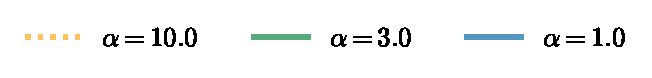
\includegraphics[width=0.4\textwidth]{new_plots_nov4/legends/fig2a.pdf}\\[0.1em]
    \vspace{-10pt}
    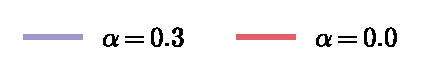
\includegraphics[width=0.25\textwidth]{new_plots_nov4/legends/fig2b.pdf}\\[0.1em]
    
    \begin{subfigure}[t]{0.24\textwidth}
        \centering
        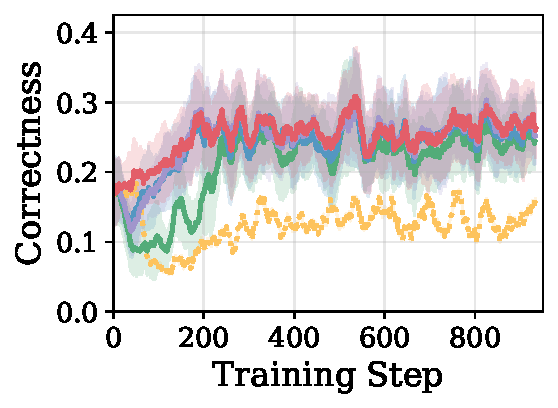
\includegraphics[width=\textwidth]{new_plots_nov4/alpha-training-plots/bl32_bernoulli_gsm8k_correctness_smooth.pdf}
    \end{subfigure}%
    \begin{subfigure}[t]{0.24\textwidth}
        \centering
        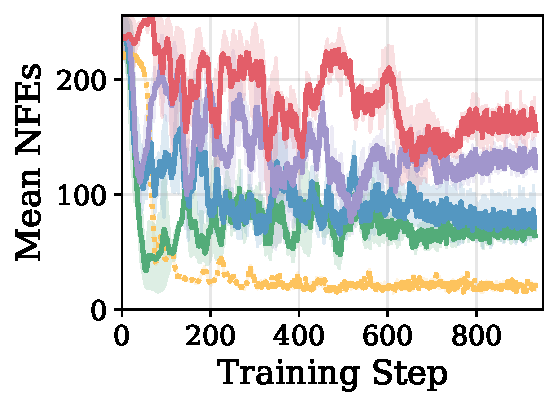
\includegraphics[width=\textwidth]{new_plots_nov4/alpha-training-plots/bl32_bernoulli_alpha_comparison_num_steps_mean.pdf}
    \end{subfigure}

    \caption{Correctness reward (rolling average, 20 steps) on GSM8k (\emph{left}) and average number of sampling steps (\emph{right}) during training of our policies for various values of $\alpha$ (cf. \Cref{eq:reward}). Averaged over two random seeds, with shaded areas indicating (min, max); only one seed shown for $\alpha = 10.0$ (\protect\yellowdottedline) due to training instability.}
    \label{fig:rl-training}
\end{wrapfigure}

\paragraph{Experiment details.} We use LLaDA-8B-Instruct \citep{llada2025} as the base dLLM (additional results on Dream-7B-Instruct \citep{ye2025dream} provided in Appendix \ref{sec:app-dream}). Note that while LLaDA is trained as an MDM from scratch, Dream is initialized from an AR model (Qwen 2.5; \citealt{qwen2025qwen25technicalreport}). We parametrize the policy network $f_{\phi}$ as a shallow (single-layer) transformer incorporating adaptive layer normalization for conditioning;
hyperparameter details for the architecture are provided in \Cref{sec:appendix_config}. We train five different policies, corresponding to $\alpha \in \{10, 3, 1, 0.3, 0\}$. Each policy is trained semi-autoregressively at $BL=32$ on a single epoch of mixture data, sampled proportionally from the training sets of GSM8k \citep{cobbe2021gsm8k} and MATH \citep{hendrycksmath2021}, resulting in roughly 15,000 training samples. \Cref{fig:rl-training} shows the training dynamics for these runs; as expected, higher $\alpha$ generally gives rise to faster policies.

We then compare the resulting policies on the test sets of both GSM8k and MATH to the confidence-based heuristics introduced in \Cref{sec:back_heuristics}, averaging over two training seeds and three test-time seeds. To obtain Pareto frontiers for the heuristic methods, we use $K \in \{8, 16, 32,64,128, 256 \}$ for the random baseline and high-confidence unmasking, while for Fast-dLLM we use $\lambda \in \{0.1, 0.2, \ldots,1.0\}$ throughout. For all methods, we use the standard greedy decoding setting ($\tau = 0$) when generating test answers. To measure sampling speed, we report the mean number of function evaluations (NFEs) of the underlying dLLM.

\paragraph{Results with (Short) 32 Block Length, \autoref{fig:gsm8k-bl32-llada} and \autoref{fig:math500-bl32-llada}}
Generally, we observe that the performance of the learned policies (\greenline)
exceeds those of both the random baseline (\greyline) as well as the high-confidence sampling (\blueline) strategy,
while matching that of Fast-dLLM (\orangeline).
The fact that our learned policies do not surpass Fast-dLLM in the mid-to-high NFEs range may suggest that this heuristic is near-optimal under the semi-AR sampling regime, where spatial correlation is enforced during the decoding process.

We note that the effect of $\alpha$ in training (cf. \Cref{fig:rl-training}) carries over to the generation on test set: policies trained with higher values of $\alpha$ exhibit faster, yet less accurate, sampling.
Of particular note is $\alpha=10.0$, which exhibited greater training instability with only 1 out of 2 training runs converging. When the seed that does take off is evaluated,
we find that it yields a very fast policy that outperforms Fast-dLLM in the low-NFE ($\sim10$) regime on both datasets. This highlights the potential of RL policies when optimizing for maximal efficiency. However, RL policies appear to exhibit less \emph{controllability} compared to a heuristic like Fast-dLLM, as varying $\alpha$ results in a less smooth traversal of the Pareto frontier than varying the confidence threshold $\lambda$.
For example, the behavior of the $\alpha = 3.0$ policy is nearly identical to that of $\alpha = 1.0$, despite the reward function incorporating a computational penalty that scales exponentially with $\alpha$.
Furthermore, we find that this cannot easily be remedied by using a tighter grid for $\alpha$.
In Appendix \ref{sec:app-alpha} we let $\alpha$ range in $ 
\{10.0, 9.0, ... 1.0, 0.3, 0.0\}$,
but observe that using $\alpha \geq 4.0$ consistently results in converging to a policy either roughly equivalent to that of $\alpha=3.0$ or to that of $\alpha=10.0$, with no value of $\alpha$ successfully yielding a policy which interpolates between the two extremes.
Besides $\alpha$, we observe that one can make small changes to the trade-off between compute and performance by varying the policy temperature $\tau_{\pi}$ at test time; we detail the impact of this parameter in \autoref{fig:bl32-test-time-temp}. %

\subsection{Beyond Semi-Autoregressive Decoding}
\label{sec:exp-bl256}
As mentioned in \Cref{sec:back_heuristics}, heuristic sampling methods often rely on semi-AR generation to achieve good performance. While not typically thought of as problematic in textual domains where strong AR dependencies exist, semi-AR approaches can only partially fulfill the promise of fully parallel generation.
Having verified that RL can help learn sampling policies with short block-length, we consider in section longer blocks.


\begin{figure}[t]
    \centering
    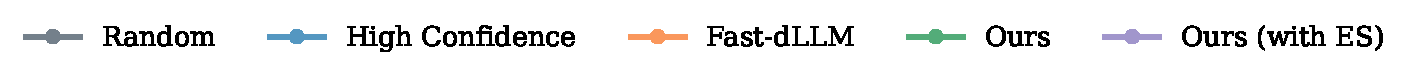
\includegraphics[width=0.95\textwidth]{new_plots_nov4/legends/fig3.pdf}

    \vspace{0.3cm}

    \begin{subfigure}[t]{0.24\textwidth}
        \centering
        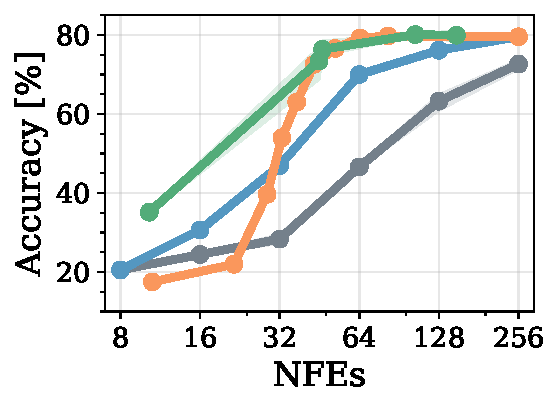
\includegraphics[width=\textwidth]{new_plots_nov4/bl32/bl32-llada-gsm8k-temp0.5.pdf}
        \caption{GSM8k, $BL=32$}
        \label{fig:gsm8k-bl32-llada}
    \end{subfigure}
    \hfill
     \begin{subfigure}[t]{0.24\textwidth}
        \centering
        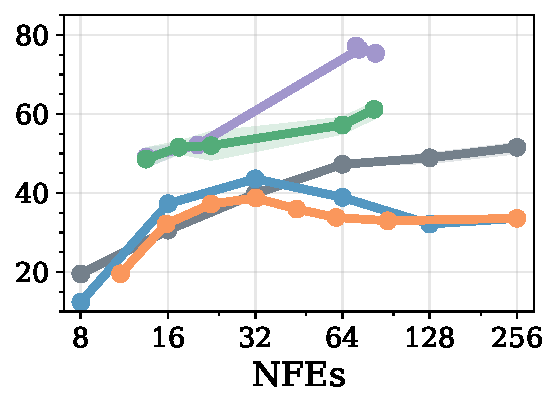
\includegraphics[width=\textwidth]{new_plots_nov4/bl256/bl256-with-wwfdd-llada-gsm8k-temp1.0-bernoulli.pdf}
        \caption{GSM8k, $BL=256$}
        \label{fig:gsm8k-bl256-llada}
    \end{subfigure}
    \hfill
    \begin{subfigure}[t]{0.24\textwidth}
        \centering
        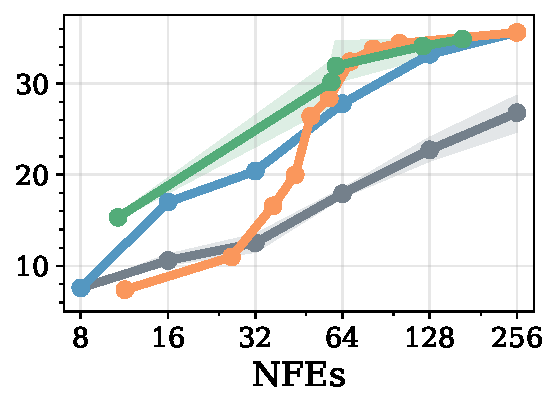
\includegraphics[width=\textwidth]{new_plots_nov4/bl32/bl32-llada-math-temp0.5.pdf}
        \caption{MATH-500, $BL=32$}
        \label{fig:math500-bl32-llada}
    \end{subfigure}
    \hfill
    \begin{subfigure}[t]{0.24\textwidth}
        \centering
        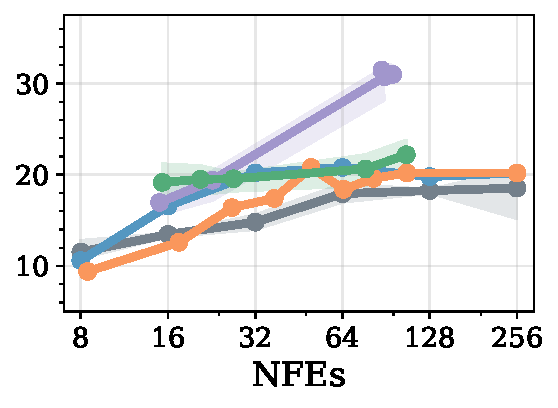
\includegraphics[width=\textwidth]{new_plots_nov4/bl256/bl256-with-wwfdd-llada-math-temp1.0-bernoulli.pdf}
        \caption{MATH-500, $BL=256$}
        \label{fig:math500-bl256-llada}
    \end{subfigure}

      \caption{Results for LLaDA in semi-AR (\Cref{fig:gsm8k-bl32-llada} \& \Cref{fig:math500-bl32-llada}) and full-diffusion (\Cref{fig:gsm8k-bl256-llada} \& \Cref{fig:math500-bl256-llada}) generation regimes. Results for Dream-7B are provided in \autoref{fig:combined-results-dream}. For our policies we vary $\alpha \in \{10, 3, 1, 0.3, 0 \}$ and use $\tau_{\pi}=0.5$ for $BL=32$ and $\tau_{\pi} = 1$ for $BL=256$. Expert steering (ES) described in detail in \autoref{sec:appendix-es}.}
      
    \label{fig:combined-results}
\end{figure}


\paragraph{Experiment details.}
We train policies without relying on semi-AR generation, targeting the full-length generation task ($BL=L=256$) at both training and test time.
We keep all other implementation details identical to those in the previous section (\Cref{sec:exp-bl32}), and evaluate on the test sets of GSM8k and MATH.

\paragraph{Results with (Long) 256 Block Length, \autoref{fig:gsm8k-bl256-llada} \& \autoref{fig:math500-bl256-llada}}
Although all sampling strategies experience a performance drop relative to the semi-AR setting (cf. \autoref{fig:gsm8k-bl32-llada} \& \autoref{fig:math500-bl32-llada}), we find that the policies produced by RL (\greenline) exhibit the smallest decline and consequently achieve the best overall performance.
Furthermore, the results suggest that this methodology is able to produce policies which achieve solid performance even in the low-NFE regime.
In particular, the learned policies obtain $\sim 50\%$ accuracy at $\sim12$ NFEs on GSM8k (compared to $\leq30\%$ for the heuristic methods regardless of semi-AR use), highlighting the potential of non-semi-AR sampling for achieving maximal efficiency gains. Note however that, in theory, a RL policy trained with $BL=L$ could learn to emulate semi-AR sampling on its own. Thus, the fact that policies trained with $BL=L$ underperform those trained with $BL=32$ in the mid-high NFE range (comparing, for example, \Cref{fig:gsm8k-bl32-llada} to \Cref{fig:gsm8k-bl256-llada}) suggests that the policies remain far from optimal.
One hypothesis for why this is the case is that our training procedure is not encouraging sufficient exploration, instead converging to locally optimal policies.
To address this, we explore encouraging further exploration by using samples generated via semi-AR sampling from Fast-dLLM.
We refer to this approach as \emph{expert steering}, and describe it in more detail in \autoref{sec:appendix-es}.
As shown in \Cref{fig:combined-results}, with expert steering (\purpleline) RL is able to discover policies that close the performance gap to the best accuracy achieved in the semi-AR setting at mid-to-high NFEs (e.g., $\sim 80\%$ on GSM8k and $\sim 35\%$ on MATH),
while mostly retaining their strong performance in the low-NFE regime.
However, we do find that expert steering introduces significant instability during training, further reducing the controllability through $\alpha$, with multiple values of $\alpha$ collapsing to near-identical policies.
We leave further investigations into stabilizing expert steering training for future work.





\subsection{Transferability of RL Sampling Policies}
\label{sec:exp-transfer}

We next turn to the question of transferability. A notable advantage of heuristic approaches like Fast-dLLM is that they can be applied \emph{post-hoc} to any model or dataset.\footnote{Though heuristics might still require manual hyperparameter tuning as exemplified by different optimal threshold across datasets for Fast-dLLM (e.g., comparing \Cref{fig:gsm8k-bl32-llada} vs \Cref{fig:humaneval-bl32-llada}).} This naturally raises the question: to what extent can RL policies trained on a specific model and dataset be reused on other models/datasets?

\paragraph{Model transfer: LLaDA $\rightarrow$ Dream.}
We begin by investigating to what extent the policies found via RL transfer across models;
note that such transfers are possible because our policies rely solely on token confidences and are therefore agnostic to token embeddings, which would not transfer from one model to another.
We thus reuse the policies trained on the LLaDA-8B-Instruct model (under the semi-AR setting; cf. \Cref{sec:exp-bl32}) and evaluate them on Dream-7B-Instruct; the results are shown in \Cref{fig:gsm8k-transfer} (see \Cref{fig:model-transfer} for MATH). 
Encouragingly, most of the LLaDA-trained policies nearly match the performance of Fast-dLLM when evaluated on Dream, and perform very similarly to those trained on Dream directly (\autoref{fig:combined-results-dream}). The one exception is the $\alpha = 10$ policy (\protect\scalerel*{\usebox{\boxgreen}}{\square}), which collapses to Fast-dLLM performance and fails to retain the good low-NFE performance observed with LLaDA (cf. \Cref{fig:gsm8k-bl32-llada})—suggesting that the extreme steepness of the reward curve (due to high $\alpha$) causes this policy to overfit to model-specific patterns in LLaDA's confidence levels. %

\paragraph{Domain transfer: Mathematical reasoning to code.}
Next, we examine how well our policies transfer across different data domains.
We again reuse the policies from \Cref{sec:exp-bl32}, which were trained on a mixture of mathematical data (GSM8K/MATH), but this time evaluate them on the coding tasks of HumanEval \citep{chen2021evaluating} and MBPP \citep{austin2021program}.
As shown in \Cref{fig:humaneval-bl32-llada} and \Cref{fig:mbpp-bl32-llada} (\greenline), we find that these policies fail to fully transfer to the coding domains: their performance more closely aligns with the high-confidence baseline rather than with Fast-dLLM.
To investigate whether this drop in performance is due to the lack of domain-relevant training data,
we train a new policy on the coding dataset KodCode-RL-10K \citep{xu2025kodcode} (\yellowline).
These coding-specific policies narrow the gap to the Fast-dLLM baseline on HumanEval and MBPP, underscoring the importance of using a diverse data mixture to support generalization across domains.
We leave to future work the training of sampling policies on mixtures that combine datasets from different domains (e.g., mathematics and coding).

\begin{figure}[t]
    \centering
    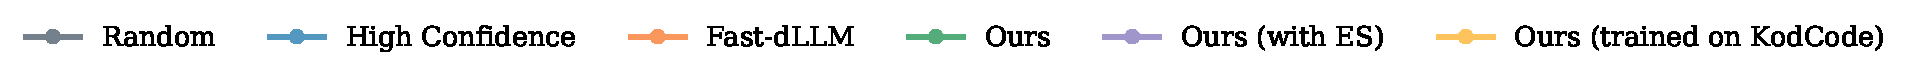
\includegraphics[width=0.95\textwidth]{new_plots_nov4/legends/fig4.pdf}

    \vspace{0.3cm}

    \begin{subfigure}[t]{0.24\textwidth}
        \centering
        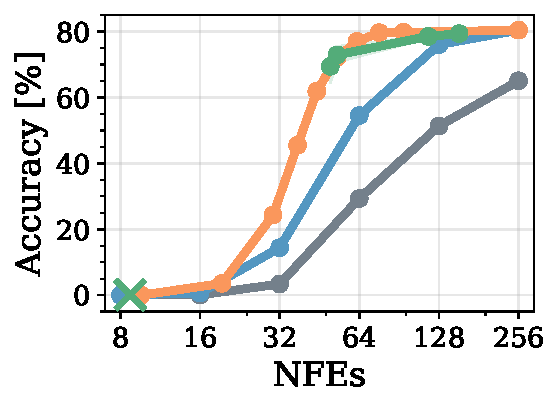
\includegraphics[width=\textwidth]{new_plots_nov4/model-transfer/llada-to-dream-bl32-gsm8k-temp0.5.pdf}
        \caption{Model transfer: LLaDA $\to$ Dream on GSM8k.}
        \label{fig:gsm8k-transfer}
    \end{subfigure}
    \hfill
    \begin{subfigure}[t]{0.24\textwidth}
        \centering
        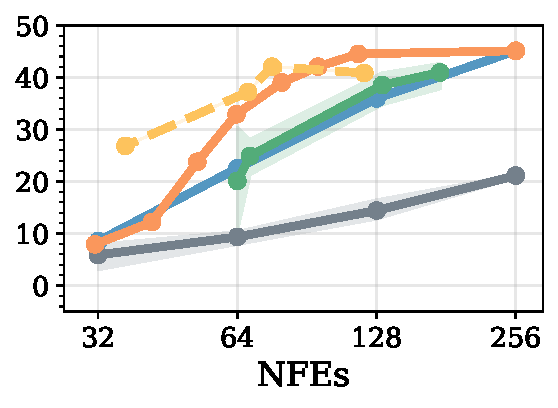
\includegraphics[width=\textwidth]{new_plots_nov4/ablation-kodcode/kodcode-ablation-humaneval-temp0.5.pdf}
        \caption{Domain transfer: math $\to$ coding (HumanEval).}
        \label{fig:humaneval-bl32-llada}
    \end{subfigure}
    \hfill
     \begin{subfigure}[t]{0.24\textwidth}
        \centering
        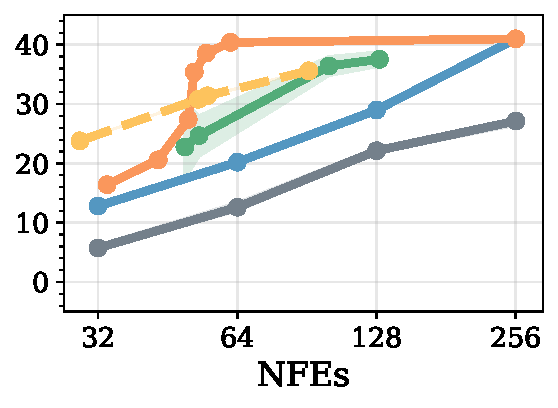
\includegraphics[width=\textwidth]{new_plots_nov4/ablation-kodcode/kodcode-ablation-mbpp-temp0.5.pdf}
        \caption{Domain transfer: math $\to$ coding (MBPP).}
        \label{fig:mbpp-bl32-llada}
    \end{subfigure}
    \hfill
    \begin{subfigure}[t]{0.24\textwidth}
        \centering
        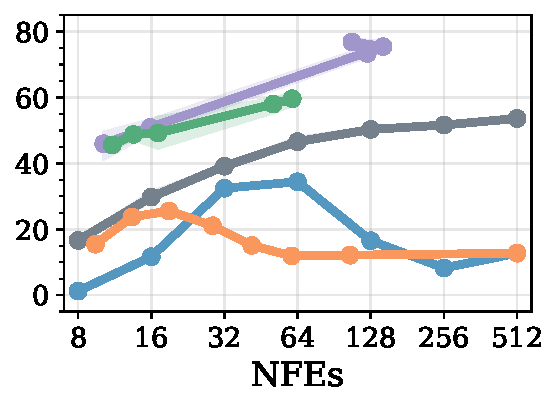
\includegraphics[width=\textwidth]{new_plots_nov4/length-transfer/bl256-to-bl512-llada-gsm8k-temp1.0.pdf}
        \caption{Sequence length transfer: $256 \to 512$ on GSM8k.}
        \label{fig:gsm8k-seq-length-transfer}
    \end{subfigure}

    \caption{Results for the transferability experiments. Note that in \textbf{(a)}, the $\alpha=10$ policy is represented separately by a (\protect\scalerel*{\usebox{\boxgreen}}{\square}) in the lower left  to avoid misleading visualization when interpolating to $\alpha=3$. For results on coding datasets in \textbf{(b)} and \textbf{(c)}, we omit the low-NFE regime, as all approaches degrade to near-zero performance in this setting.}
    \label{fig:transfer-comparison}
\end{figure}

\paragraph{Sequence length generalization: $L=256 \to L=512$.}
Lastly, we examine whether our policies transfer across different sequence lengths $L$ (not to be confused with the block length $BL$ used in semi-AR generation).
Such transfer is possible since we instantiate $f_\theta$ with a transformer trained with rotary positional embeddings \citep{su2021roformer}, rather than, for example, an MLP or other fixed-length architectures.
We thus take the policies from \Cref{sec:exp-bl256} and evaluate them at a 2x longer sequence length, $L=512$.
Results are shown in \Cref{fig:gsm8k-seq-length-transfer} (see \autoref{fig:length-transfer} for MATH results). While the baselines degrade further as the sequence length increases, the learned policies yield similar performance to before, suggesting that RL policies can transfer effectively across generation lengths without retraining.



\subsection{Exploring the Design Space of $\pi_\phi$}
\label{sec:exp-ablate}
Lastly, we conduct a series of experiments to elucidate the impact of various design choices behind our proposed RL sampling method.

\paragraph{Additive vs. multiplicative rewards}
We begin by ablating the structure of the reward function, comparing our proposed multiplicative combination of correctness and computational terms (cf. \Cref{eq:reward}) with an additive alternative: $r(\vy, \vy_{\hat{T}})- \alpha \big(\frac{T - \hat{T}}{T} \big)$.
As shown in \Cref{fig:reward-ablation}, while both exhibit increasing reward as training progresses, we observe that the additive formulation is much more prone to `reward hacking', where it collapses to a very-fast-but-very-wrong policy.
This is illustrated in \Cref{fig:reward-ablation-num-steps}: training with the additive reward results in a policy that unmasks everything at once, leading to the number of sampling steps to collapse to the minimum possible for all samples (i.e., $8$ steps for training with $BL=32$ and $L=256$).
As discussed in \Cref{sec:methods_grpo}, we attribute this issue to the fact that incorrect but fast samples may still receive a positive advantage under the additive reward. %
In contrast, we find that the multiplicative reward effectively mitigates this issue by assigning a positive advantage only if the generation is correct, resulting in more stable and predictable training behavior.

\paragraph{Policy likelihood}
Next, we examine our choice of the policy likelihood parameterization. Recall from \Cref{sec:methods_policy} that we model the unmasking probability for each position using a Bernoulli distribution. 
This has the advantage of admitting very efficient inference and likelihood calculations, but relies on the network $f_\phi$ to implicitly embed relationships between different tokens in the scores $\vb_t$, and runs the risk of producing $\gU_t^{\pi} = \emptyset$ in case $\vu_t = \mathbf{0}$.
In this experiment, we therefore investigate a more involved sampling procedure, which we call \emph{dynamic Plackett-Luce sampling} (DPLS; detailed description in \autoref{sec:appendix-dpls}) which is guaranteed to unmask at least one position in each step and which non-linearly combines the scores $\vb_t$ through a softmax, while still allowing for variable-size unmasking sets $\gU_t^{\pi}$.
Since this affects not only the sampling strategy but also the likelihood computation, we retrain the policies from \Cref{sec:exp-bl32}; the resulting downstream accuracy on GSM8k is then showed in \autoref{fig:sampling-ablation-gsm8k-rls}. We observe that both methods achieve very similar performance, aligning closely with the Fast-dLLM frontier, which might provide additional support for the hypothesis that this frontier is optimal in the semi-AR setting.
Furthermore, DPLS policies appear to show slightly better controllability via $\alpha$ parameter (as indicated by a larger spread of policies trained with varying $\alpha$). 

\paragraph{Confidence-based policy input} 
Finally, we revisit our design choice of relying solely on the maximum token confidence values $c_t^k$ as input to the sampling policy (cf. \Cref{sec:methods_policy}) to explore whether other measures of uncertainty in the base model's predictions could yield better results. We first train and evaluate a set of policies which do not take only the highest confidence per position $c_t^k$ as input, but rather the top 50 highest values, thus giving the model more detailed information about the token predictive distributions $p_t^k$ and potentially allowing it to design its own confidences measures for effective sampling. The results are presented in \Cref{fig:sampling-ablation-top-50}.
Somewhat surprisingly, using only the maximum confidence per position (\greenline) performs slightly better than using the top-50 confidences (\purpleline), which suggests that alternative uncertainty measures are unlikely to yield performance gains over the simple confidences $c_t^k$. 

\begin{figure}[t]
    \centering
    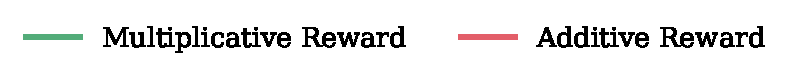
\includegraphics[width=0.45\textwidth]{new_plots_nov4/legends/fig5a.pdf}
    \hspace{5ex}
    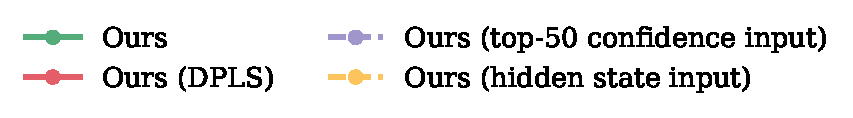
\includegraphics[width=0.45\textwidth]{new_plots_nov4/legends/fig5b.pdf}


    \begin{subfigure}[t]{0.24\textwidth}
        \centering
        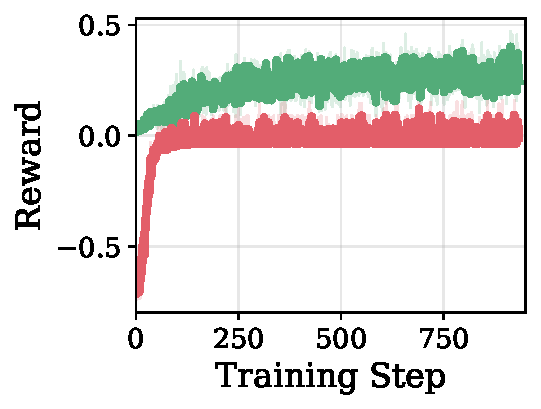
\includegraphics[width=\textwidth]{new_plots_nov4/ablation-reward/reward.pdf}
        \caption{Training reward for LLaDA with additive vs. multiplicative reward function (both $\alpha = 1.0$).} 
        \label{fig:reward-ablation}
    \end{subfigure}
    \hfill
    \begin{subfigure}[t]{0.24\textwidth}
        \centering
        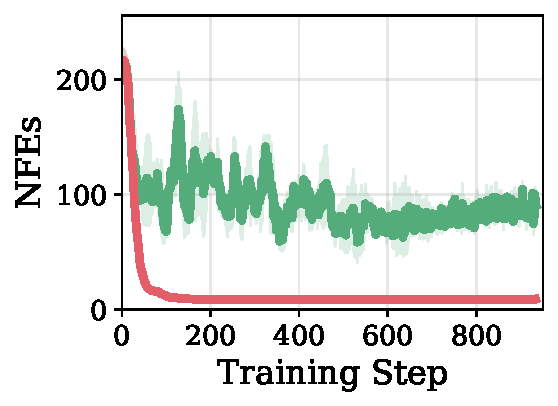
\includegraphics[width=\textwidth]{new_plots_nov4/ablation-reward/num_steps_mean.pdf}
        \caption{Mean number of NFEs when training LLaDA with additive vs. multiplicative reward (both $\alpha = 1.0$).}
        \label{fig:reward-ablation-num-steps}
    \end{subfigure}
    \hfill
    \begin{subfigure}[t]{0.24\textwidth}
        \centering
        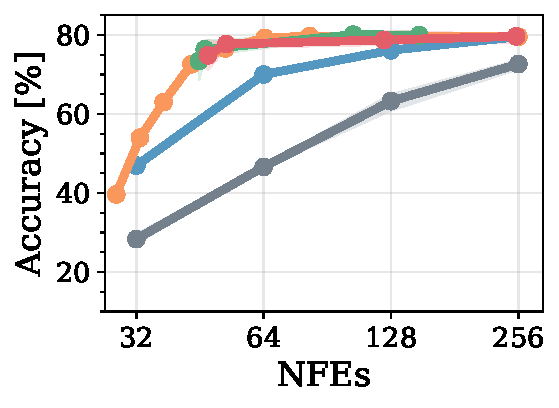
\includegraphics[width=\textwidth]{new_plots_nov4/ablation-rls/bl32-rls-llada-gsm8k-temp0.5.pdf}
        \caption{Bernoulli vs DPLS sampling on GSM8k. Both for LLaDA on GSM8k, $\tau_{\pi}=0.5$.}
        \label{fig:sampling-ablation-gsm8k-rls}
    \end{subfigure}
    \hfill
     \begin{subfigure}[t]{0.24\textwidth}
        \centering
        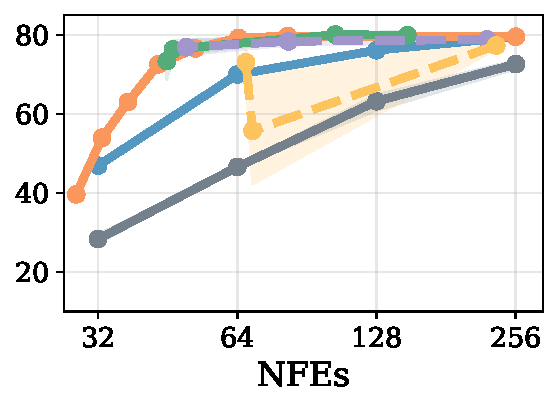
\includegraphics[width=\textwidth]{new_plots_nov4/ablation-topk/bl32-top50-ablation-gsm8k-temp0.5.pdf}
        \caption{Bernoulli policy with top-1 versus with top-50 confidences. Both for LLaDA on GSM8k, $\tau_{\pi}=0.5$.}
        \label{fig:sampling-ablation-top-50}
    \end{subfigure}
    \caption{Ablations for our proposed RL framework.}
    \label{fig:ablations}
\end{figure}

Additionally, we consider parametrizing the policy as an additional classification head on top of LLaDA's final hidden state $\vh_t^k \in \mathbb{R}^H$.
While this results in a significantly larger policy ($300M$ parameters, an increase of $1,000\times$), it offers the potential advantage of incorporating token-level semantic information. However, in practice we observe that hidden state-based policies perform worse (see \yellowline~in \Cref{fig:sampling-ablation-top-50}) and exhibit less stable training dynamics than the confidence-based policies. These results suggest that the unembedding matrix $W \in \mathbb{R}^{H \times V}$, which maps hidden states to token logits, plays a vital role in enabling effective policy decisions via confidence signals.\footnote{Similar findings have been reported in the early-exit literature \citep{schuster2022confident}, where confidence-based stopping criteria have been shown to significantly outperform those relying on hidden state representations.}

